%capitulo 5 pagina 38%
    \begin{frame}{Ejemplo: 4-reinas}
        \textcolor{Green}{Estados:} 4 reinas en 4 columnas (\textcolor{Purple}{$4^4=256$}) estados\\
        \textcolor{Green}{Operadores:} mover la reina en columna\\
        \textcolor{Green}{Objetivo de ensayo:} sin ataques\\
        \textcolor{Green}{Evaluación:} \textcolor{Purple}{$h(n)$} = numero de ataques
        \begin{figure}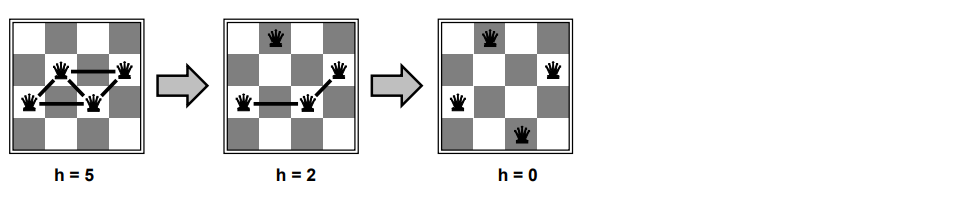
\includegraphics[width =120mm]{38img.png}\end{figure}
        
    \end{frame}